\section{Machine Learning Workloads} \label{sec-ml-workloads}
We define a machine learning workload as a series of exploratory data analysis steps followed by one or multiple model building steps.
Typically users analyze the data by first performing an exploratory analysis.
Then, based on these analyses, they apply the right set of transformations to the data to train one or multiple models on the transformed training data.
Therefore, machine learning workloads typically consist of both interactive (exploratory analysis) and long-running processes (hyperparameter tuning and model training).
Using the experiment database, we can speed up the execution of the machine learning workloads.
By analyzing the experiment database, we can extract the common transformations on data and materialize them.
Thus, during the interactive exploratory analysis, we first analyze the workload to look for reuse opportunities and return the materialized data when possible.
Moreover, using the experiment database, we provide the users with already trained models or promising hyperparameters which decreases the execution time of the hyperparameter search and model training.

We analyzed several scripts from the Titanic: Machine Learning from Disaster competition in Kaggle\footnote{https://www.kaggle.com/c/titanic}.
The Kaggle platform allows users to submit their solutions as scripts (called notebooks or kernels) to the Kaggle platform.
These notebooks are available publicly for other users to view and fork in their own workspace.
Figure \ref{fig-titanic-script-hierarchy} shows some of the popular notebooks and how other users wrote their notebooks based on the existing ones.
The numbers show how many times each script is forked.
The top most-voted notebooks for the Titanic competition have been forked a total of 44,434 times.
This demonstrates that many of the workloads share similar sets of data transformations and model training.
Materializing frequent transformations and models can greatly increase the efficiency and many repeated operations can be avoided.

\begin{figure}
\centering
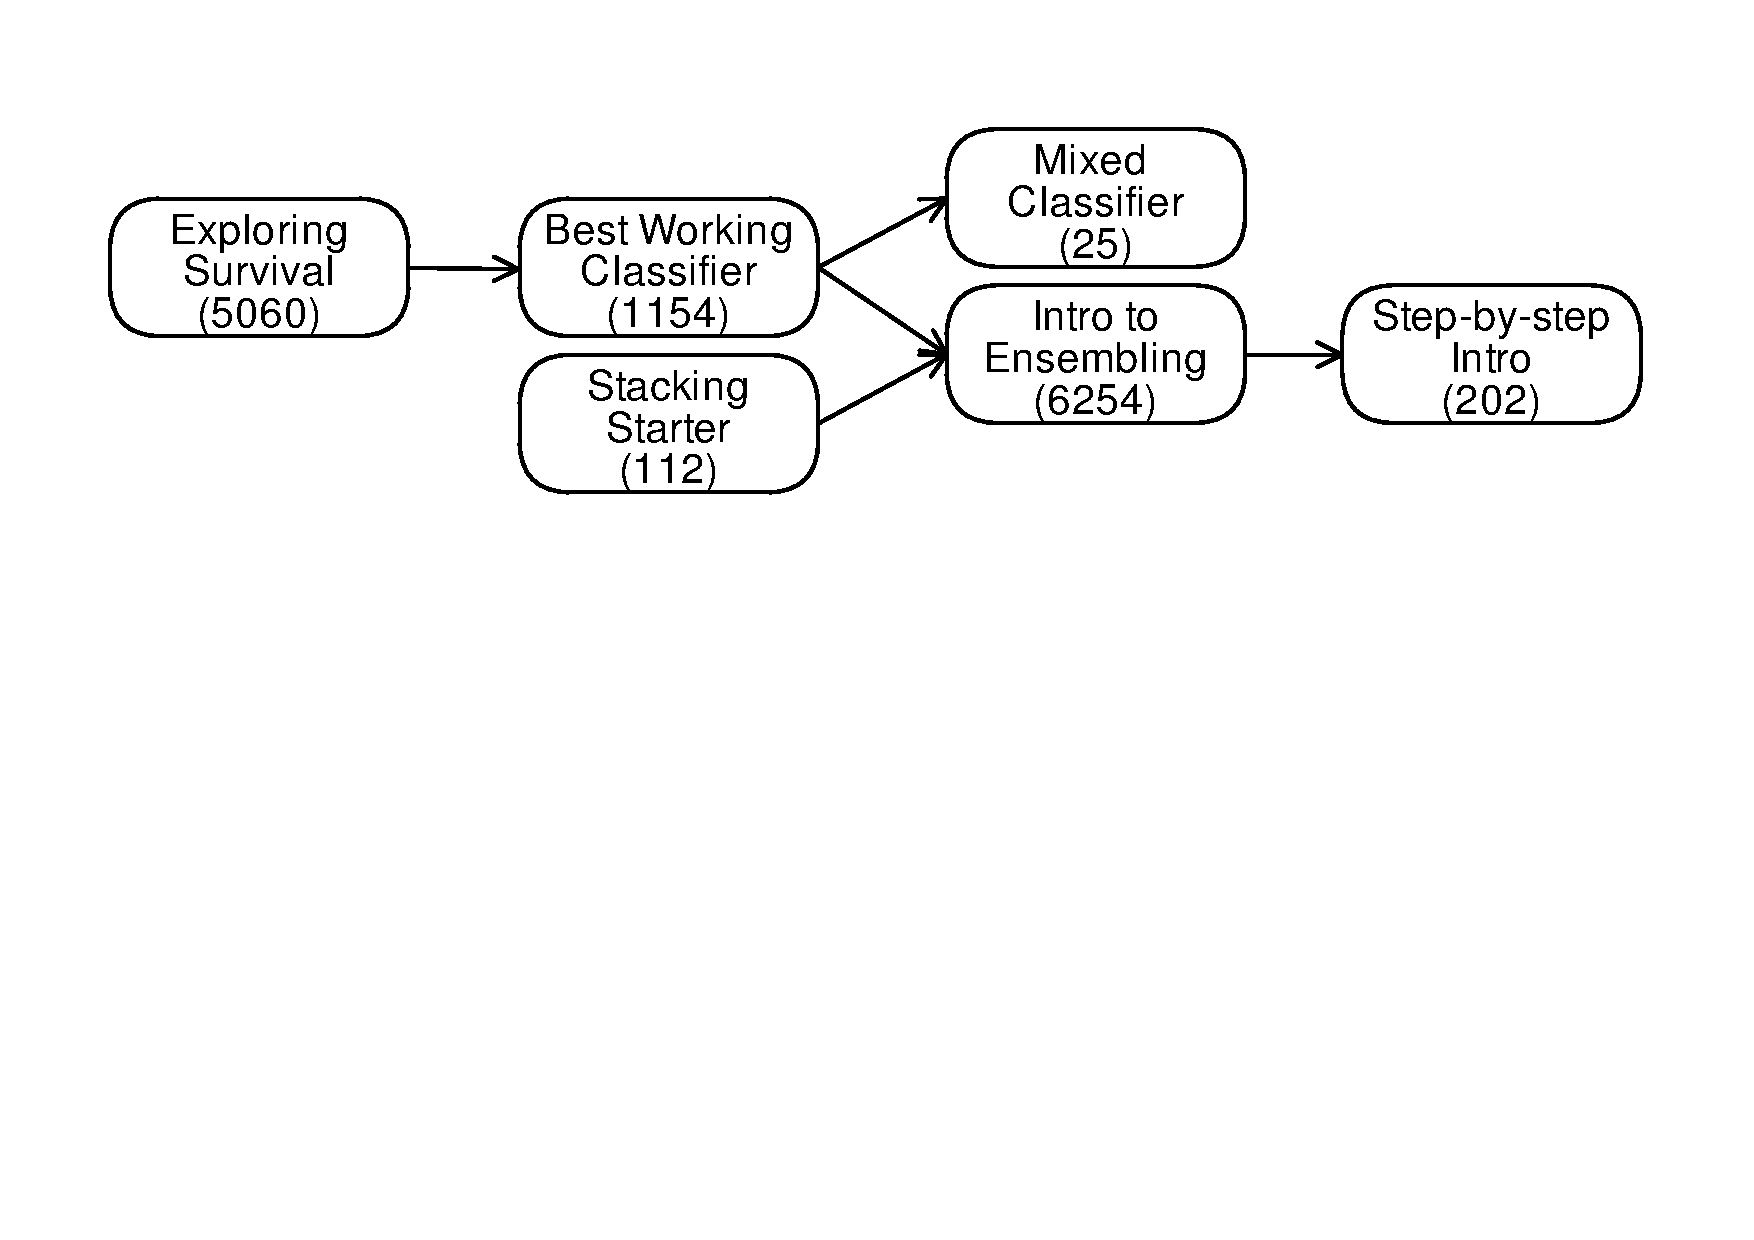
\includegraphics[width=\columnwidth]{../images/kaggle-titanic-scripts-graph}
\caption{The fork hierarchy of some of the popular notebooks in Kaggle's Titanic competition and how many times each notebook is forked}
\label{fig-titanic-script-hierarchy}
\end{figure}

In order to apply the materialization optimization, we first define the characteristics of the interactive machine learning workloads.
Then, we specify how to detect reuse opportunities from the experiment database.

\subsection{Machine Learning Workload Characteristics}
We assume the main units of work are dataframe like objects that contain one or many columns, where all the data items in one column are of one data type.
We divide the operations in interactive ML workloads into 2 categories.

\textbf{1. Feature engineering:}
\begin{itemize}
\item feature selection operation that selects a set of features (columns) from the dataset
\item feature transformation that applies a function to a set of columns from the dataset and generates new columns
\end{itemize}


\textbf{2. Model building: }
\begin{itemize}
\item model training that applies a training algorithm to a dataset
\item aggregation operation that aggregates a set of columns based on the values in another column
\end{itemize}
Each model building operation results in objects (vertices) that can either be used in other feature engineering operations (applying PCA to data or categorization the data based on percentile values) or can be a complete machine learning model that can be used to make predictions on unseen data.
\todo[inline]{How can we capture these in the graph? maybe special edges that connect these nodes to a data node? }

\todo[inline]{In the rest of this section, I only mention materialization for the feature engineering operations. I have some ideas for the model building operations as well, but I will skip that for now. }

%%% Continue from here
\subsection{Graph Construction}
To construct the experiment graph, we first analyze each feature engineering and model building operation to create the vertices and edges of the graph.
A feature engineering transformation operation is defined as \textit{transform(d, i\_columns, tf, o\_columns)}, where $d$ represents the dataset, $i\_columns$ represents the list of input columns, $tf$ represents the function to be applied to those columns, and $o\_columns$ represents the output columns (selection operation can be defined as a transform operation as well). 
In the graph, vertices represent datasets and transformation operations that transform one dataset to another dataset, represent edges.
Each vertex node contains a reference to the dataset and the list of the columns that the dataset contains.
Each edge contains the transformation function ($tf$) and the list of the input columns ($i\_columns$).

We define the model building operations with two methods.
Training a machine learning model is defined as \textit{train(d, alg)} which trains a model using the $alg$ on the given data $d$.
An aggregation operations is defined as \textit{aggr(d, i\_columns, af)}, which performs a $groupby$ on the input columns ($i\_columns$) and aggregate the groups using the $af$ function.

Figure \ref{fig-experiment-graph} shows an example graph constructed from the code in Listing \ref{listing-experiment-graph}.
The script is based on the \textit{Titanic Best Working Classifier} from the Kaggle competition\footnote{https://www.kaggle.com/sinakhorami/titanic-best-working-classifier}.

\begin{lstlisting}[language=Python, caption=Example script,captionpos=b,label = {listing-experiment-graph}]
import numpy as np
import pandas as pd
from sklearn.tree import DecisionTreeClassifier

train = pd.read_csv('../input/train.csv')
print (train[['Pclass', 'Survived']].groupby(['Pclass']).mean())
train['IsAlone'] = 0
train.loc[dataset['FamilySize'] == 1, 'IsAlone'] = 1
train['Embarked'] = train['Embarked'].fillna('S') 
train['Sex'] = train['Sex'].map( {'female': 0, 'male': 1} )
train_matrix = train.values
model = DecisionTreeClassifier()
model.fit(train_matrix)
\end{lstlisting}

\begin{figure}
\centering
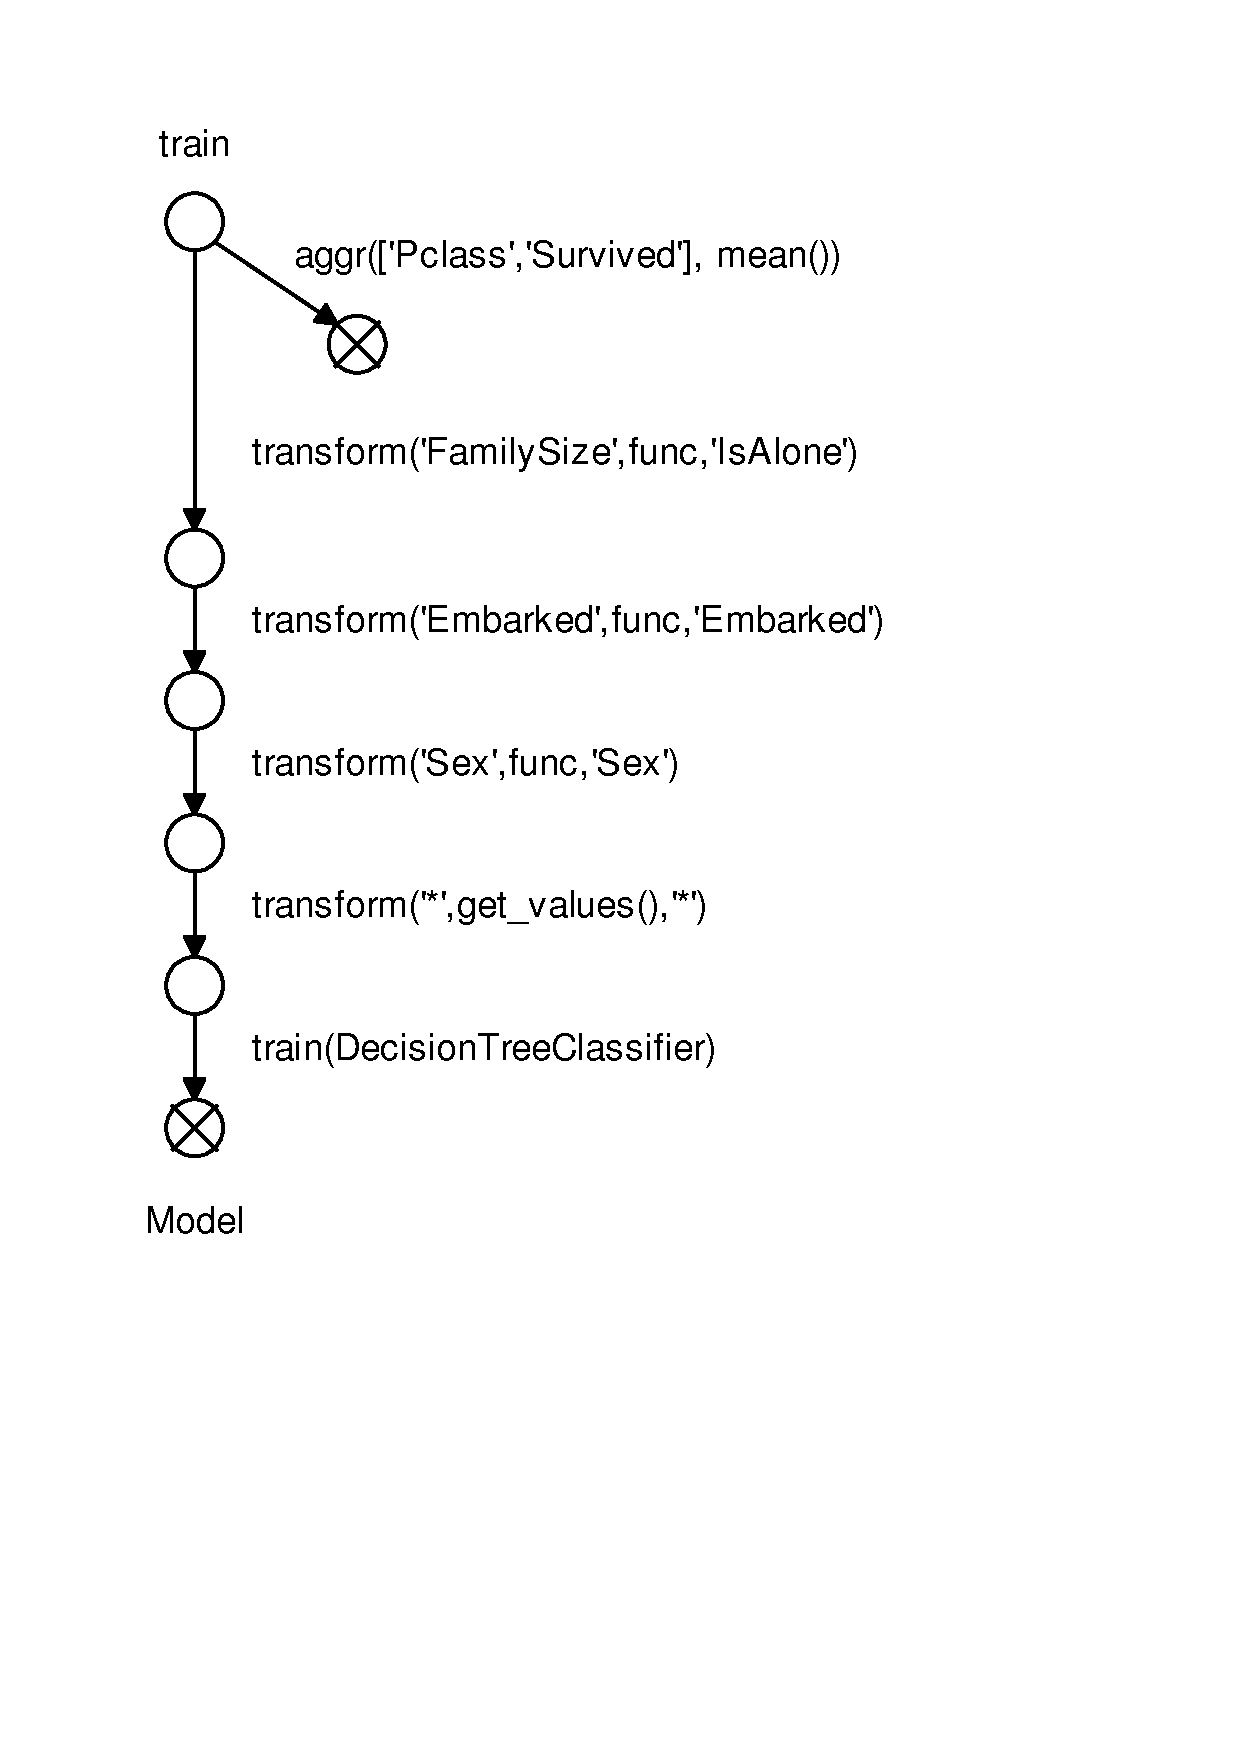
\includegraphics[width=0.6\columnwidth]{../images/experiment-graph}
\caption{Experiment graph constructed from the Listing \ref{listing-experiment-graph}}
\label{fig-experiment-graph}
\end{figure}
